\documentclass[twoside]{report}

% Page & text layout
\usepackage[twoside]{geometry}
\geometry{%
  a4paper,%
  top=30mm,%
  bottom=30mm,%
  left=30mm,%
  right=20mm%
}
\usepackage[utf8]{inputenc}
\usepackage[T1]{fontenc}
\usepackage{lmodern}
\usepackage[ngerman]{babel}
\usepackage{amsmath} % für Mathematische Formeln
\usepackage{titling} % um die Befehle \theauthor zu haben.
\usepackage{ulem}   % zum durchstreichen von text.

\usepackage{graphicx}
\usepackage{caption}
\usepackage{subcaption}

\parindent0pt % sorgt dafür, dass neue Absätze nicht eingerückt werden.

%%% DOXYGEN Commandos

% Packages required by doxygen
\usepackage{calc}
\usepackage{doxygen}
\usepackage{graphicx}
\usepackage[utf8]{inputenc}
\usepackage{makeidx}
\usepackage{multicol}
\usepackage{multirow}
\usepackage{textcomp}
\usepackage[table]{xcolor}

% Font selection
\usepackage{mathptmx}
\usepackage[scaled=.90]{helvet}
\usepackage{courier}
\usepackage{amssymb}
\usepackage{sectsty}
\renewcommand{\familydefault}{\sfdefault}
\allsectionsfont{%
  \fontseries{bc}\selectfont%
  \color{darkgray}%
}
\renewcommand{\DoxyLabelFont}{%
  \fontseries{bc}\selectfont%
  \color{darkgray}%
}

\tolerance=750
\hfuzz=15pt
\hbadness=750
\setlength{\emergencystretch}{15pt}
\setlength{\parindent}{0cm}
\setlength{\parskip}{0.2cm}
\makeatletter
\renewcommand{\paragraph}{%
  \@startsection{paragraph}{4}{0ex}{-1.0ex}{1.0ex}{%
    \normalfont\normalsize\bfseries\SS@parafont%
  }%
}
\renewcommand{\subparagraph}{%
  \@startsection{subparagraph}{5}{0ex}{-1.0ex}{1.0ex}{%
    \normalfont\normalsize\bfseries\SS@subparafont%
  }%
}
\makeatother

% Indices & bibliography
\usepackage{natbib}
\usepackage[titles]{tocloft}
\setcounter{tocdepth}{3}
\setcounter{secnumdepth}{5}
\makeindex

\newcommand{\clearemptydoublepage}{%
  \newpage{\pagestyle{empty}\cleardoublepage}%
}

%%% DOXYGEN Ende



\usepackage{listings}
\usepackage[german,vario]{fancyref}

% Headers & footers
\usepackage{fancyhdr}
\pagestyle{fancyplain}
\fancyhead[LE]{\fancyplain{}{\bfseries\thepage}}
\fancyhead[CE]{\fancyplain{}{}}
\fancyhead[RE]{\fancyplain{}{\bfseries\leftmark}}
\fancyhead[LO]{\fancyplain{}{\bfseries\rightmark}}
\fancyhead[CO]{\fancyplain{}{}}
\fancyhead[RO]{\fancyplain{}{\bfseries\thepage}}
\fancyfoot[LE]{\fancyplain{}{\bfseries\scriptsize \theauthor}}
\fancyfoot[CE]{\fancyplain{}{}}
\fancyfoot[RE]{\fancyplain{}{\bfseries\scriptsize Dokumentation zu Flächennutzungsregeln }}
\fancyfoot[LO]{\fancyplain{}{\bfseries\scriptsize Dokumentation zu Flächennutzungsregeln }}
\fancyfoot[CO]{\fancyplain{}{}}
\fancyfoot[RO]{\fancyplain{}{\bfseries\scriptsize \theauthor}}
\renewcommand{\footrulewidth}{0.4pt}
\renewcommand{\chaptermark}[1]{%
  \markboth{#1}{}%
}
\renewcommand{\sectionmark}[1]{%
  \markright{\thesection\ #1}%
}

% Hyperlinks (required, but should be loaded last)
\usepackage{ifpdf}
\ifpdf
  \usepackage[pdftex,pagebackref=true]{hyperref}
\else
  \usepackage[ps2pdf,pagebackref=true]{hyperref}
\fi
\hypersetup{%
  colorlinks=true,%
  linkcolor=black,%
  citecolor=black,%
  unicode%
}

% Custom commands
\def\signed #1{{\leavevmode\unskip\nobreak\hfil\penalty50\hskip2em
  \hbox{}\nobreak\hfil(#1)%
  \parfillskip=0pt \finalhyphendemerits=0 \endgraf}}

\newsavebox\mybox
\newenvironment{aquote}[1]
  {\savebox\mybox{#1}\begin{quote}}
  {\signed{\usebox\mybox}\end{quote}}

\title{Dokumentation zu \\[.5\baselineskip] Flächennutzungsregeln}
\author{Fabian Pflug  |  Peter Zilz}
\date{\today}

%===== C O N T E N T S =====

\begin{document}

% Titlepage & ToC
\setcounter{secnumdepth}{5}
\setcounter{tocdepth}{2}
\hypersetup{pageanchor=false}
\pagenumbering{roman}

% Titelseite
\pagestyle{empty}
\begingroup
\hbox{ % Horizontal box
\hspace*{0.2\textwidth} % Whitespace to the left of the title page
\rule{1pt}{\textheight} % Vertical line
\hspace*{0.05\textwidth} % Whitespace between the vertical line and title page text
\parbox[b]{0.75\textwidth}{ % Paragraph box which restricts text to less than the width of the page

{\noindent\Huge\bfseries \thetitle }\\[2\baselineskip] % Title
{\large \textit{Gruppe InMa}}\\[4\baselineskip] % Tagline or further description
{\Large \textsc{\theauthor}} % Author name

\vspace{0.5\textheight} % Whitespace between the title block and the publisher
{\noindent \thedate}\\[\baselineskip]
{\noindent Leibniz Universität Hannover}\\[\baselineskip] % Publisher and logo
}}
\endgroup


\clearpage
\begin{abstract}
Der Abstrakt mit einer Zusammenfassung aller Sachen die wir gemacht haben/machen werden.

\end{abstract}

\cleardoublepage
\setcounter{page}{1}
\pagestyle{fancy}
\tableofcontents

\cleardoublepage
\pagenumbering{arabic}
\hypersetup{pageanchor=true}

\cleardoublepage
\chapter{Erste Runde}
\section{Grundüberlegungen}
Aus den Beispielen im Text lässt sich ableiten, dass es sinnvoll ist 'nicht rauchen' Gebiete eher in Bereiche zu legen, welche Gebäude representieren,
oder alternativ Parkplätze bei der Berechnung auszublenden.

\subsection{Testdatensatz}
\label{sec:Testdatensatz}
Zunächst wurde der Testdatensatz mithilfe von Google Maps, Google Street View, Google Earth und OpenStreetMap auf Richtigkeit, Machbarkeit der Lösungen und eventuelle Fehler überprüft.
Im Testdatensatz lassen sich etliche Fehler und Unvollständigkeiten finden. So sind für die Datensätze:
\begin{itemize}
\item 33 (nur teilweise)
\item 34 (nur teilweise)
\item 36
\item 38
\item 39
\item 41
\item 43 - 45
\item 49 (nur teilweise)
\item 50 (nur teilweise)
\item 53
\item 55 - 62
\end{itemize}
keine Representationen der beabsichtigten Geltungsbereiche in OpenStreetMap vorhanden.
\newline
\\
Weitere Fehler sind:
\begin{itemize}
\item 16 Der Bereich müsste größer sein.
\item 33 Sollte den selben Bereich abdecken wie 24.
\item 40 Es ist kein Häuserblock gemeint, sonder nur ein einzelnes Haus auf der gegenüberliegenden Strassenseite.
\item 43 Der reale Bereich ist etwas verschoben.
\item 51 Der reale Bereich liegt auf der gegenüberliegenden Strassenseite.
\item 55 Das gewählte Gebäude ist falsch. Das reale befindet sich weiter westlich.
\item 57 Das Bild zeigt das Gebäude, welches bei Bild 41 abfotografiert wurde.
\item 59 Das Bild suggestiert, dass das Parkverbot in dem Strassenabschnitt vor dem Gebäude gilt und nicht in diesem, da es sich um ein Wohnhaus handelt.
\item 84 Das Bild suggestiert einen anderen Bereich, als auf Google Maps angezeigt wird. (in Maps ist kein See erkennbar.)
\item 85 Das Bild zeigt ein 'Betreten Verboten' Schild mit Schienen im Hintergrund und sollte dementsprechend für den Schienenbereich gelten und nicht für das Bahnhofsgebäude.
\item 90 Das Verbot sollte nur für ein einzelnen Haus gelten.
\item 93 Das Verbot gilt sinnvollerweise für den Zoo und nicht ein einzelnes Gebäude.
\item 96 Das 'Betreten Verboten im Brandfall' gilt nur für den Fahrstuhl und nicht für das ganze Gebäude.
\end{itemize}

\subsection{Fehlerbehebung}
Nach Rücksprache mit Herrn Porada, sowie Herrn Schöning haben sich einige Fehler klären lassen.
\begin{itemize}
\item Die Fehler in 16, 33 und 59 wurden berichtigt.
\item Bei 93 wurde geklärt, dass das Schild nur für ein einzelnes Zoogebäude gelten darf/kann, da im Zoo das teilweise füttern der Tiere erlaubt ist.
\item Für 96 wurde es dabei belassen, dass man ein ganzes Haus nimmt.
\item Für 40 und 85 hat sich keine Übereinstimmung der Interpretation finden lassen. Diese werden von uns bei der Auswertung der Testdatensätze nicht berücksichtigt.
\item Für die Restlichen wurden die Fehler als Aufnahmeunschärfe erklärt und werden nicht weiter hinterfragt sondern als richtig angenommen.
\end{itemize}


\subsection{Erweiterung der Testdaten}
Da in dem Testdatensatz so viele Fehler vorhanden sind, ist geplant diesen zu erweitern. Dazu wird eine Android-App programmiert, in welcher Nutzer SpaceUsageRules
abhängig von ihrer Position angezeigt bekommen und sie neue hinzufügen können.
Um die Qualität unserer bisherige Regeln zu überprüfen, und dem Benutzer die Eingabe zu vereinfachen, wird ein Vorschlag gemacht,
welchen er annehmen oder abändern kann. Auch soll es ihm möglich sein einen komplett neuen Bereich einzeichnen zu können.
Die angelegten Daten werden anschließend mit OpenStreetMap synchronisiert, sodass sich für die Nutzer auch ein eigener Nutzen ergibt
und sie ein Ergebnis ihres Beitrages sehen.
Für jede angelegte Regel werden Nutzungsdaten an uns übertragen, die aus der Position des Nutzers, des Menge an Verbotsnamen sowie des angelegten Bereiches besteht.
Wir erhoffen uns daraus einen Testdatensatz zu bekommen, welcher um den Faktor 5 bis 10 größer ist und es uns erlaubt die erstellten Regeln effizienter zu überprüfen.

\section{Regeln}

\subsection{Formale Beschreibung:}
Sei $ID$ die die Bezeichnung eines Bildes.\\
Sei $t$ ein Tag $(key \to value)$ aus OpenStreetMap.\\
Sei $r(t)$ eine Regel $t \to [0..2]$ \\
Sei $Z_{X}$ die Menge der Tag $t$ für die Gilt: $t$ kommt in X vor. \\
Sei $R_v$ eine Menge von Funktionen $r$ für das Verbot $v$\\
Sei $C_{ID}$ die Geocoordinate, an welcher das Bild zu $ID$ aufgenommen wurde. \\
Sei $D_{X,ID}$ der Abstand eines Polygons $X$ zu $C_{ID}$ \\
Sei $O_{ID}$ eine Menge von Polygonen aus OpenStreetMap in der Umgebung zu $C_{ID}$\\
Sei $A_{X}$ die Fläche des Polygons $X$\\
Sei $V$ die Menge aller Verbote $v$.\\
Sei $V_{ID}$ die Menge der Verbote für die gilt: $v$ wird auf dem Bild zu $ID$ abgebildet.\\
Sei $S_{v}$ die Menge der $ID$ für die gilt: $v \in V_{ID}$\\
Sei $P_{ID}$ das gegebene Lösungspolygon zu $ID$.\\
Sei $I(X,Y)$ das Schnittpolygon der Polygone X und Y\\
\\
Sollte es für ein $t$ kein $r(t)$ geben, so wird die standartregel:
$r(t) = 1$ angewendet.

\begin{equation}
Gew(R,ID,X) := \sum_{v \in V_{ID}} \Big((1 + D_{X,ID})\prod_{t \in Z_X} \prod_{r \in R_v} r(t)\Big)
\end{equation}

\begin{align}
G(ID,R) := \{X \in O_{ID} | & Gew(R,ID,X) < Gew(R,ID,Y)\\
& \lor \Big(Gew(R,ID,X)=Gew(R,ID,Y) \land A_X < A_Y\Big) \forall Y\} \notag
\end{align}

\subsection{Beispiel}
Eine Regel kann z.B. so aussehen:
Für das Verbot Nichtrauchen: wenn ein Tag den Key 'building' enhält dann halbiere den Abstand. \\
$R_{nichtrauchen} = [r('building') = 0.5]$\\
\newline
Seien in der Umgebung zu $ID$ nur zwei Flächen A,B in OpenStreetMap vorhanden.
\begin{itemize}
\item A enthält die Tags: 'building -> yes', 'addr:housenumber -> 34' und hat den Abstand 0.002;
\item B enthält die Tags: 'landuse->residential' und hat den Abstand 0;
\end{itemize}
Daraus errechnet sich:
\begin{itemize}
\item $Gew(R,ID,A) = (1+0.002) * 0.5 * 1 = 0.501$
\item $Gew(R,ID,B) = (1+0.0) * 1 = 1$
\end{itemize}

$G(ID,R) = A$

\subsection{Maschinelle Überprüfung der Regelsätze}
Um die Güte der verschiedenen Regeln zu überprüfen wird ein Programm geschrieben, welche für jede Regel die die Schnittpolygone von unseren Polygonen mit
den Musterlösungen bildet und anschließen durch je die Fläche unseres Polygons, sowie des Musterlösungspolygons teilt.
Von beiden Zahlen wird das Minimun genommen und als Indicator der Lösungsgüte angesehen.\\
\begin{equation}
f(v,R) := \sum_{q\in S_v} min(\frac{I(P_q,G(q,R))}{P_q},\frac{I(P_q,G(q,R))}{G(q,R)})
\end{equation}
Um die Güte des Regelsatzes für ein einzelnes Verbot vergleichbar zu anderen Verboten zu machen wird abschließend der Indicator durch
die Anzahl der $ID$s welches es beeinflussen geteilt.\\
\begin{equation}
\label{eq:guete}
Güte(R) := \sum_{v \in V} \frac{ f(v,R)}{\#S_v}
\end{equation}

Wir suchen also einen Regelsatz $R$ für den $Güte(R)$ maximal ist.


\subsection{Visuelle Überprüfung}
\label{sec:visuelle_ueberpruefung}
Um die KML-Dateien nicht immer manuell in Google-Earth laden zu müssen, wurde eine weitere Klasse geschrieben, welche zur Visualisierung der Daten gedacht ist.
Dabei werden Bilder erstellt, in welchen die Daten aus OSM als schwarze Linien, bzw Polygone eingezeichnet werden. Zusätzlich werden die Tags, 
welche die Objekte enthalten zu jedem Objekt eingezeichnet um schnell eine Übersicht zu haben, was wozu gehört.
Um die Güte des Regeldatensatzes, bzw des Algorithmus subjektiv beurteilen zu können, werden die truth, bzw. die von unserem Algorithmus erdachten Polygone
farblich eingezeichnet. so ist eine schnelle Beurteilung, ob man das richtige Poylgon gewählt hat, bzw welche Tags man evtl noch beachten sollten möglich.

\subsection{Incrementelle Regelerstellung}
Aus dem Testdatensatz werden zunächst alle Datensätze herausgefiltert, welche nicht einfach lösbar sind.
Es wird mit einem leeren Regelsatz angefangen und dieser anschließend inkrementel erweitert. Dazu wird wie Folgt vorgegangen:
\begin{enumerate}
\item Definiere für jeden Datensatz ein optimales Polygon, bzw einen Overlap-Wert, welcher erreicht werden muss.
\item Der Regelsatz wird auf alle Testdatensätze angewendet.
\item Für jeden Datensatz, bei welchem die Regeln nicht das optimale Polygon finden, wird ein Bild wie in \fref{sec:visuelle_ueberpruefung} erstellt.
\item Dem Benutzer werden alle Bilder, angezeigt und dieser kann nun weitere Regeln hinzufügen oder bestehende ändern.
\item gehe zu 2
\end{enumerate}
Nachdem alle einfachen Fälle abgedeckt sind, kann nun mit den schwierigeren Vorgegangen werden.
Gehe dazu erneut so vor.

\subsection{Mögliche Erweiterung}
Um den Fall abzudecken, in welchem in OpenStreetMap keine ausreichenden Daten vorhanden sind, wird um den Punkt $C_{ID}$ ein
Achteck\footnote{Relativ geringer Rechenaufwand bei gleichzeitig bester Annäherung an einen Kreis.} mit Radius $b$ gelegt
und dieses mit der gewichtet nächsten Großfläche geschnitten.
Eine Großfläche X definiert sich dadurch, dass ihre Fläche $A_X$ einen schwellwert $u$ überschreitet.
Es ist zu prüfen ob es sinnvoll ist dieses generell zu tun oder für bestimmte Regel ausser kraft zu setzen wie
z.B. ein Verbot nach offenem Feuer, welches in einem ganzen Parkgebiet gelten wird.
\section{Softwareimplementierung}
Auch wenn Anfangs eine deutliche Tendenz zu C/C++ als Programmiersprache der Wahl war, fiel durch das spätere Interesse für eine
Android Applikation die Wahl auf Java. So ist es einfach möglich einen Kern mit Algorithmen zu schreiben und diesen von den
verschiedenen Anwendungen als Bibliothek nutzen zu lassen.

\subsection{Entwurf}


\subsection{Eingabeformat}
\subsubsection{Regeln}
\label{sec:Eingabedaten_Wir}
Regeln werden aus einer Textdatei eingelesen, in welcher zeilenweise die Regeln zu je einem Verbot stehen.
Die Datei besteht aus zwei Spalten, in der Ersten steht der Name des Verbotes in der Zweiten die Menge der Regeln.
Die Menge wird durch eckige Klammern verdeutlicht und die einzelnen Regeln durch Kommata getrennt.
Die Trennung von Key und Value erfolgt durch einen Bindestrich.
Soll eine Regel generell für alle Values eines Keys gelten, so kann die Value weggelassen und nur der Key angegeben werden.

Eine Gültige Eingabe kann also folgendermaßen sein:
\begin{lstlisting}[frame=single]
smoking="no" -> [addr:housenumber -> 0.5, landuse - forest -> 1.5]
fishing="no" -> []
\end{lstlisting}
Dieses Regelwerk sagt aus, dass ein Nichtrauchen Verbot wahrscheinlich in Flächen gilt, welche eine Hausnummer zugewiesen haben
und sehr unwahrscheinlich in Gebieten, die als Waldgebiete ausgeschildert sind.
Für das Angelverbot sind keine Regeln definiert. Unser Algorithmus wird sich also nur die nächstegelegene Fläche als wahrscheinlich nehmen,
oder sollten der Punkt innerhalb von 2 Flächen liegen\footnote{Es könnte z.B. eine Fläche 'Niedersachsen' und eine Fläche 'Waldgebiet' definiert sein.},
so wird die kleinere von beiden ausgewählt.

\subsubsection{Daten}
\label{sec:Eingabedaten_GI}
Hier werden die aus der Aufgabenstellung übernommenen Regeln beachtet und das Eingabeformat wie beschrieben umgesetzt.
\begin{quote}
Die erste Zeile enthält die Anzahl $c$ der Space Usage Rules. Es folgen zeilenweise die Informationen
über die $c$ Regeldefinitionen.
Eine Zeile beginnt mit der ID der Space Usage Rule gefolgt von deren Position in geographischen
Koordinaten in der Form $Breitengrad, Längengrad$. Als Eingabewerte sind für $Breitengrad$ und
$Längengrad$ Fließkommazahlen mit einem ’.’ als Dezimaltrennzeichen erlaubt. Die einzelnen Informationen
sind durch Kommas und optionale Leerzeichen getrennt.
\end{quote}

\subsection{Probleme}
Da die Berechnung der Schnittpolygone sehr aufwändig ist und wir nur eine Näherung benötigen,
wird die Berechnung der Schnittpolygone und deren Flächen vereinfach durch erstellen von Bounding Boxes.
Es wird also nicht das wirkliche Schnittpolygon berechnet, sondern die Schnitt Bounding Box, sowie die Fläche der Bounding Box.

\section{Automatisierte Regelerstellung}
Da uns die Grundaufgabe nicht informatiklastig genug ist
haben wir beschlossen unser selbst definiertes Regelwerk abschließend gegen ein Learning Classifier System antreten zu lassen.

\subsection{Eingabedaten}
\begin{itemize}
\item Eine Liste mit SpaceUsageRules wie in \fref{sec:Eingabedaten_GI} definiert.
\item Die dazugehörigen truth.kml Dateien.
\item Verschiedene Parameter zum Steuern des genetischen Algorithmus
%\footnote{Siehe auch fref{sec:Evaluation_genAlg}}
  \begin{itemize}
  \item Populationsgröße
  \item Anzahl der Verbesserungsversuche
  \item Anzahl der Populationen, welche unverändert in die nächste Generation gehen.
  \item Anzahl der Populationen, welche mutiert in die nächste Generation gehen.
  \item Anzahl der Populationen, welche mit anderen gemischt in die nächste Generation gehen.
  \end{itemize}
\end{itemize}

\subsection{Ausgabedaten}
Das System ist so entworfen, dass es als Ausgabe Daten liefert wie in \fref{sec:Eingabedaten_Wir} von unserem Algortihmus verlangt werden.

\section{Vorgehensweise}
Es werden zunächst für alle Eingabedaten die Daten im Umkreis der Positionsdaten aus Openstreetmap heruntergeladen.
Aus diesen werden alle möglichen Tags extrahiert. Tags, welche nur einmalig vorkommen, werden ignoriert, um zum einen die Menge zu verkleinern
und zum anderen die Regeln allgemeiner zu halten und sie so einfacher und besser auf andere Datensätze übertragen zu können.
Anschließend für jede Verbotsmenge ein Genetischer Algorithmus erstellt, welcher die Verbote für diesen optimiert und in einem eigenem Thread läuft.
Nachdem alle Algorithmen durchgelaufen sind, werden die Optimalen eingesammelt und aus ihnen ein Regelwerk erstellt und in eine Datei geschrieben.

\subsection{Fitnessfunktion}




\subsection[Evaluation]{Evaluation\protect\footnotemark}
\footnotetext{Es wurden nur die einfachen Datensätze ausgewertet.
Alle Durchläufe fanden auf dem selben Rechner statt (Core i5-3570K - 16GB RAM)}

\label{sec:Evaluation_genAlg}
\begin{figure}
  \begin{subfigure}[b]{\textwidth}
  \includegraphics[width=\textwidth]{LaufzeitGen90Q.png}
  \caption{Qualität}
  \end{subfigure}

  \begin{subfigure}[b]{\textwidth}
  \includegraphics[width=16cm]{LaufzeitGen90T.png}
  \caption{Laufzeit}
  \end{subfigure}
\caption{in Abhängigkeit verschiedener Paramter.}
\label{fig:GenAlgAll}
\end{figure}

Wie in \fref{fig:GenAlgAll} zu sehen ist, wird die Laufzeit und die Ergebnisse des Genetischen Algorithmus positiv beeinflusst,
wenn man den Merge-Wert möglichst hoch setzt. Kein anderer Faktor hat so einen positiven Einfluss auf das Ergebniss.
(Bei höheren Populationsgrößen steigt zwar auch die Qualität, aber gleichzeitig auch die Laufzeit im Gegensatz zum Merge-Wert)

\begin{figure}
  \begin{subfigure}[b]{\textwidth}
  \includegraphics[width=\textwidth]{LaufzeitMerge5Q.png}
  \caption{Qualität}
  \label{fig:QualitätMerge5}
  \end{subfigure}

  \begin{subfigure}[b]{\textwidth}
  \includegraphics[width=\textwidth]{LaufzeitMerge5T.png}
  \caption{Laufzeit}
  \label{fig:LaufzeitMerge5}
  \end{subfigure}
\caption{des Genetischen Algorithmus für fixen Merge-Wert von 5.\protect}
\label{fig:GenAlgMerge5}
\end{figure}

Wenn wir festlegen, dass 50\% der Populationen in der neuen Generation aus den Besten der alten zusammen gepaart werden sollen,
dann erhalten wir Ergebnisse (Siehe \fref{fig:GenAlgMerge5}), die in der Qualität sehr homogen sind und für Populationsgröße
und Wiederholungen in der Laufzeit ansteigt.
Es ist also zu vermuten, dass bereits für eine kleine Anzahl von Wiederholungen und Populationsgrößen
ein brauchbares Ergebnis erzielt werden kann.
Des weiteren ist Ersichtlich, dass die Anzahl der Populationen, welche mutiert übernommen werden sollen
keinen nennenswerten Einfluss auf die Qualität oder Laufzeit hat.



%\cleardoublepage
%\chapter{Zweite Runde}
%\section{Datenerstellung}
Die Bilder wurden am Nachmittag des 15.Januar mit einem Android Tablet erstellt.
Dieses enthält einen GPS-Sensor, sowie eine einfache Kamera.

\section{Probleme}
Beim Erstellen der Truth-Datensätze stellte sich heraus, dass der GPS-Sensor teilweise
ungenaue Positionen, welche um etliche Meter, wenn nicht sogar hunderte Meter von
der eigentlichen Position abweichen. Dieses ist im genauen Gegensatz zu den Testdatensätzen,
bei welchen die Bilder eine genauere Position lieferten, als es aus der Data.txt
herauszulesen war.

Als Lösung dieses Problems, wurde eine Überprüfung des Abstandes zwischen GPS-Koordinate
und Data.txt Koordinate implementiert, welche bei überschreiben eines Schwellwertes
die Koordinate im Bild verwirft. Es kann davon ausgegangen werden, dass Daten, welche
in die Data.txt eingetragen sind von Menschen überprüft wurden.


\section{Regelwerk}
\begin{figure}
  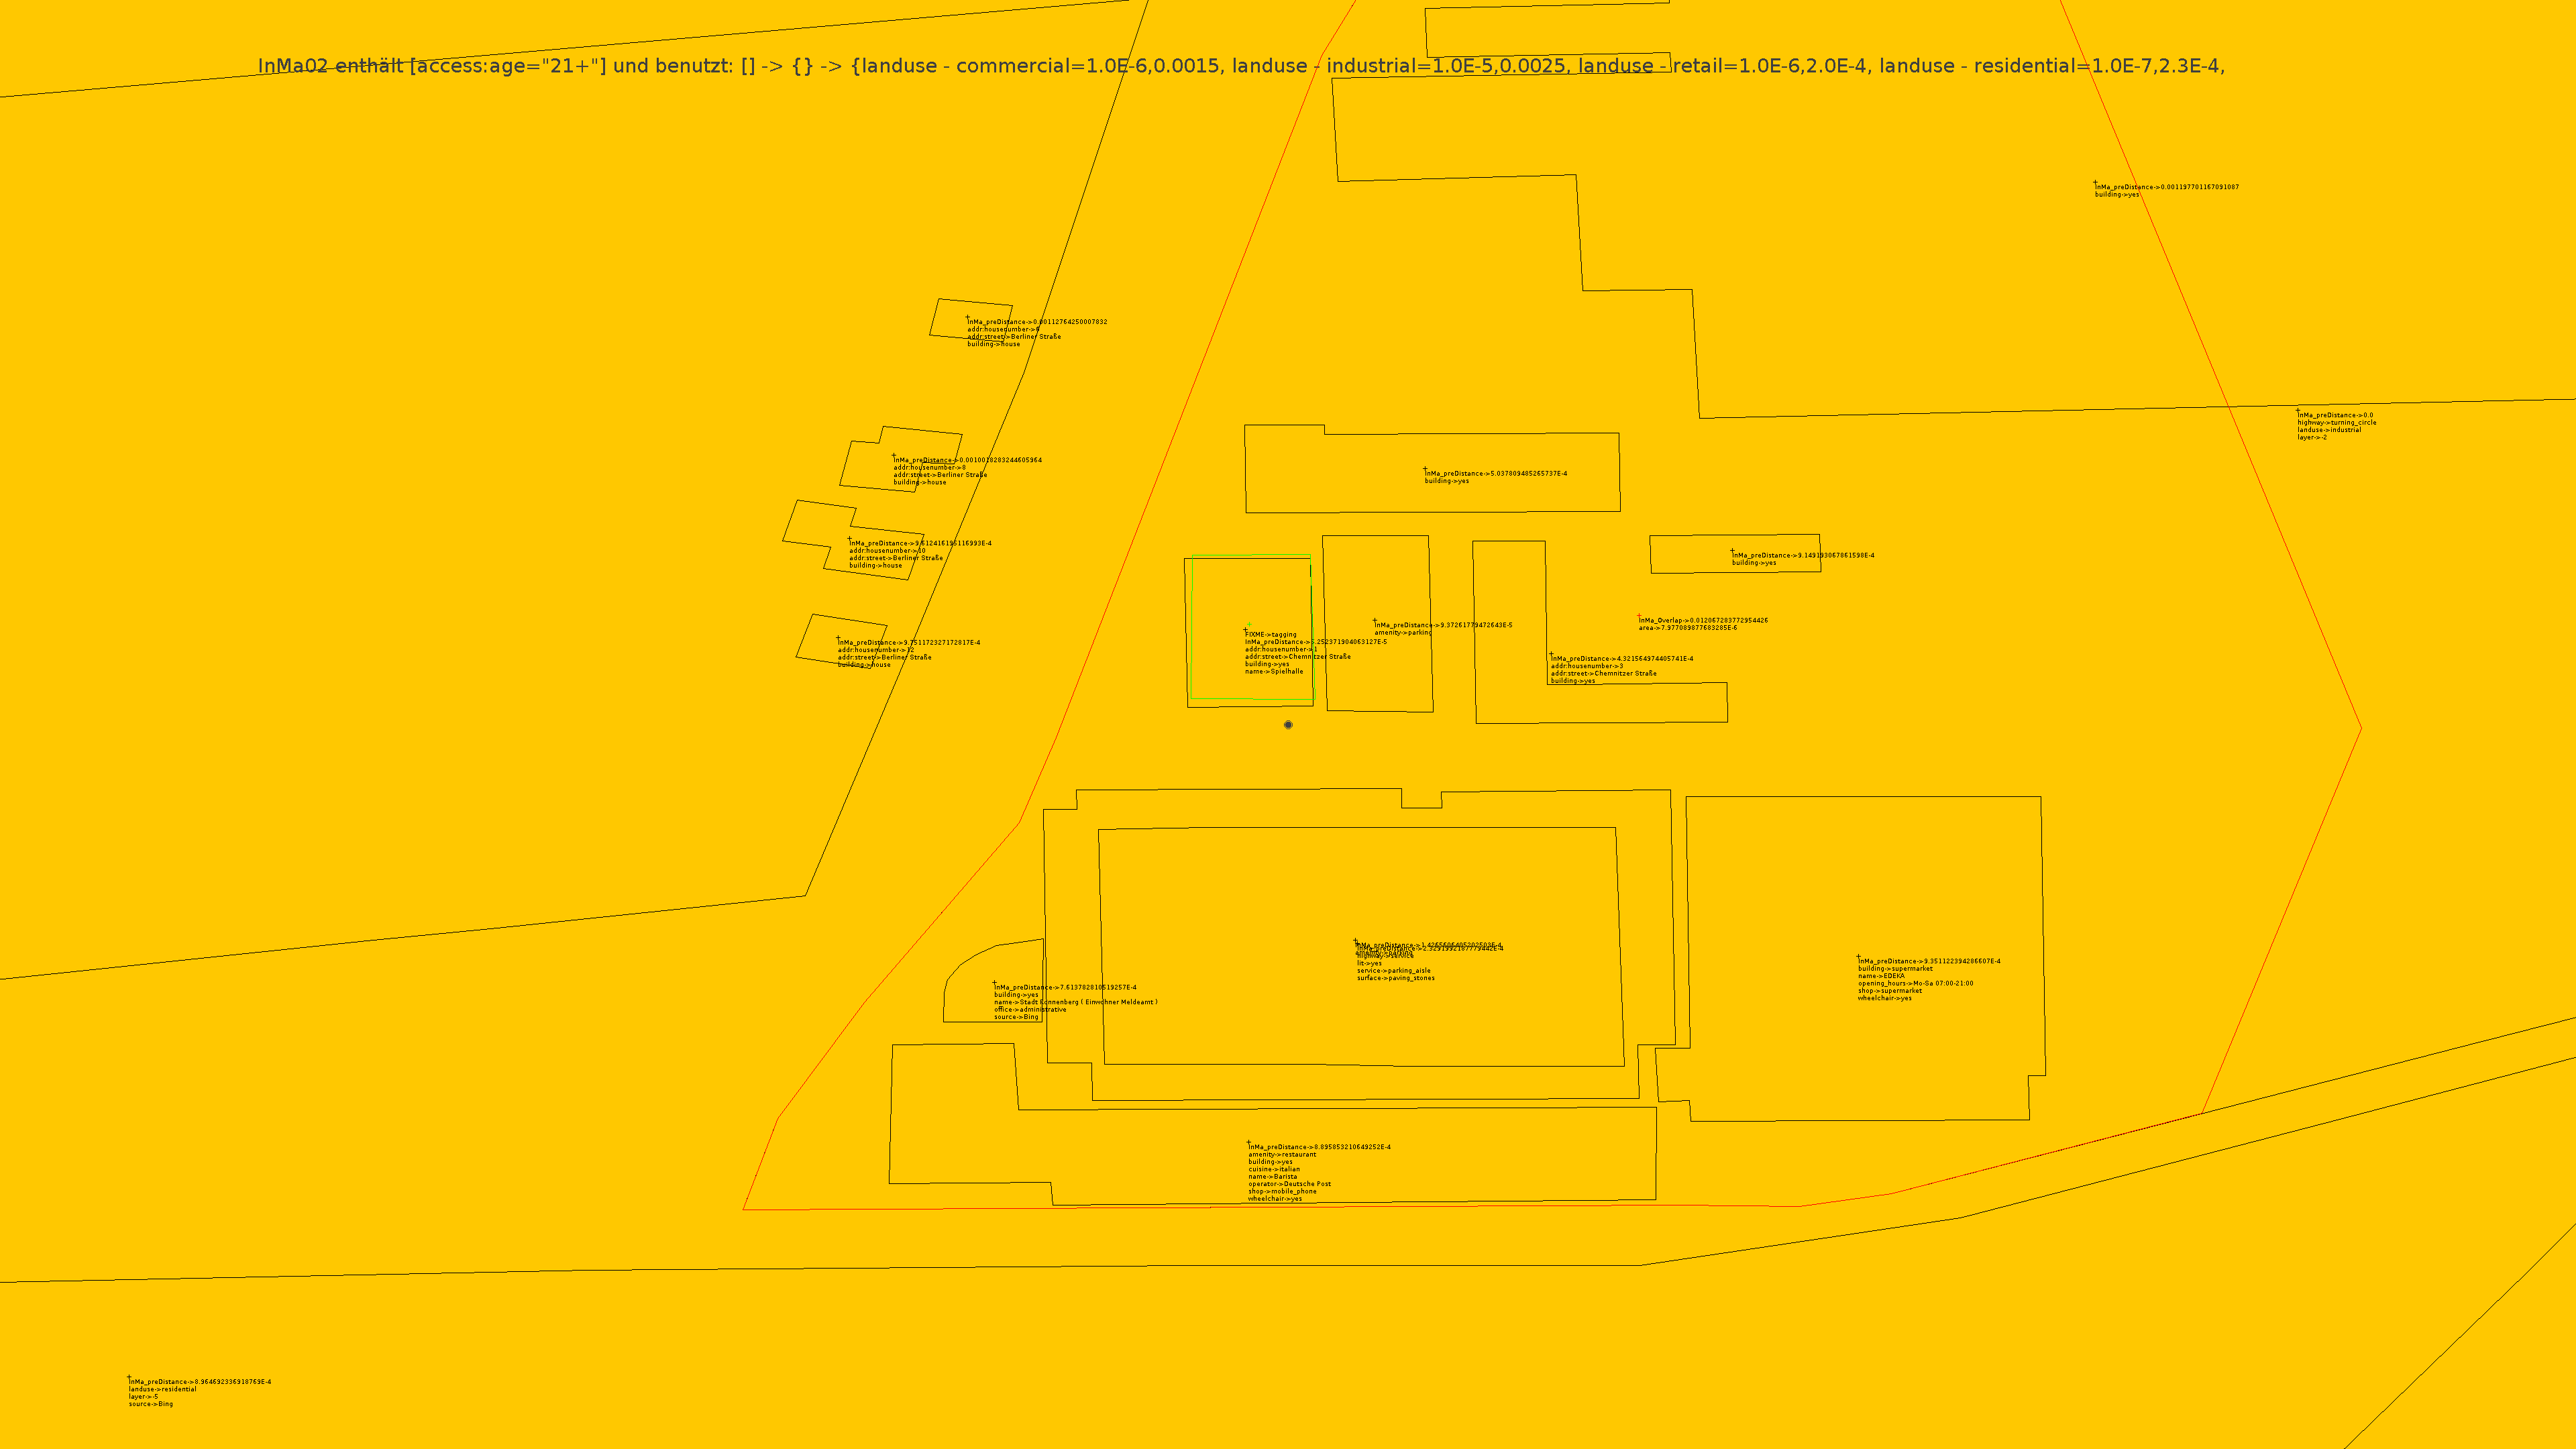
\includegraphics[width=\textwidth]{InMa02.png}
  \caption{Unvollständige Rules Definition.}
  \label{fig:NoRule}
\end{figure}

\begin{figure}
  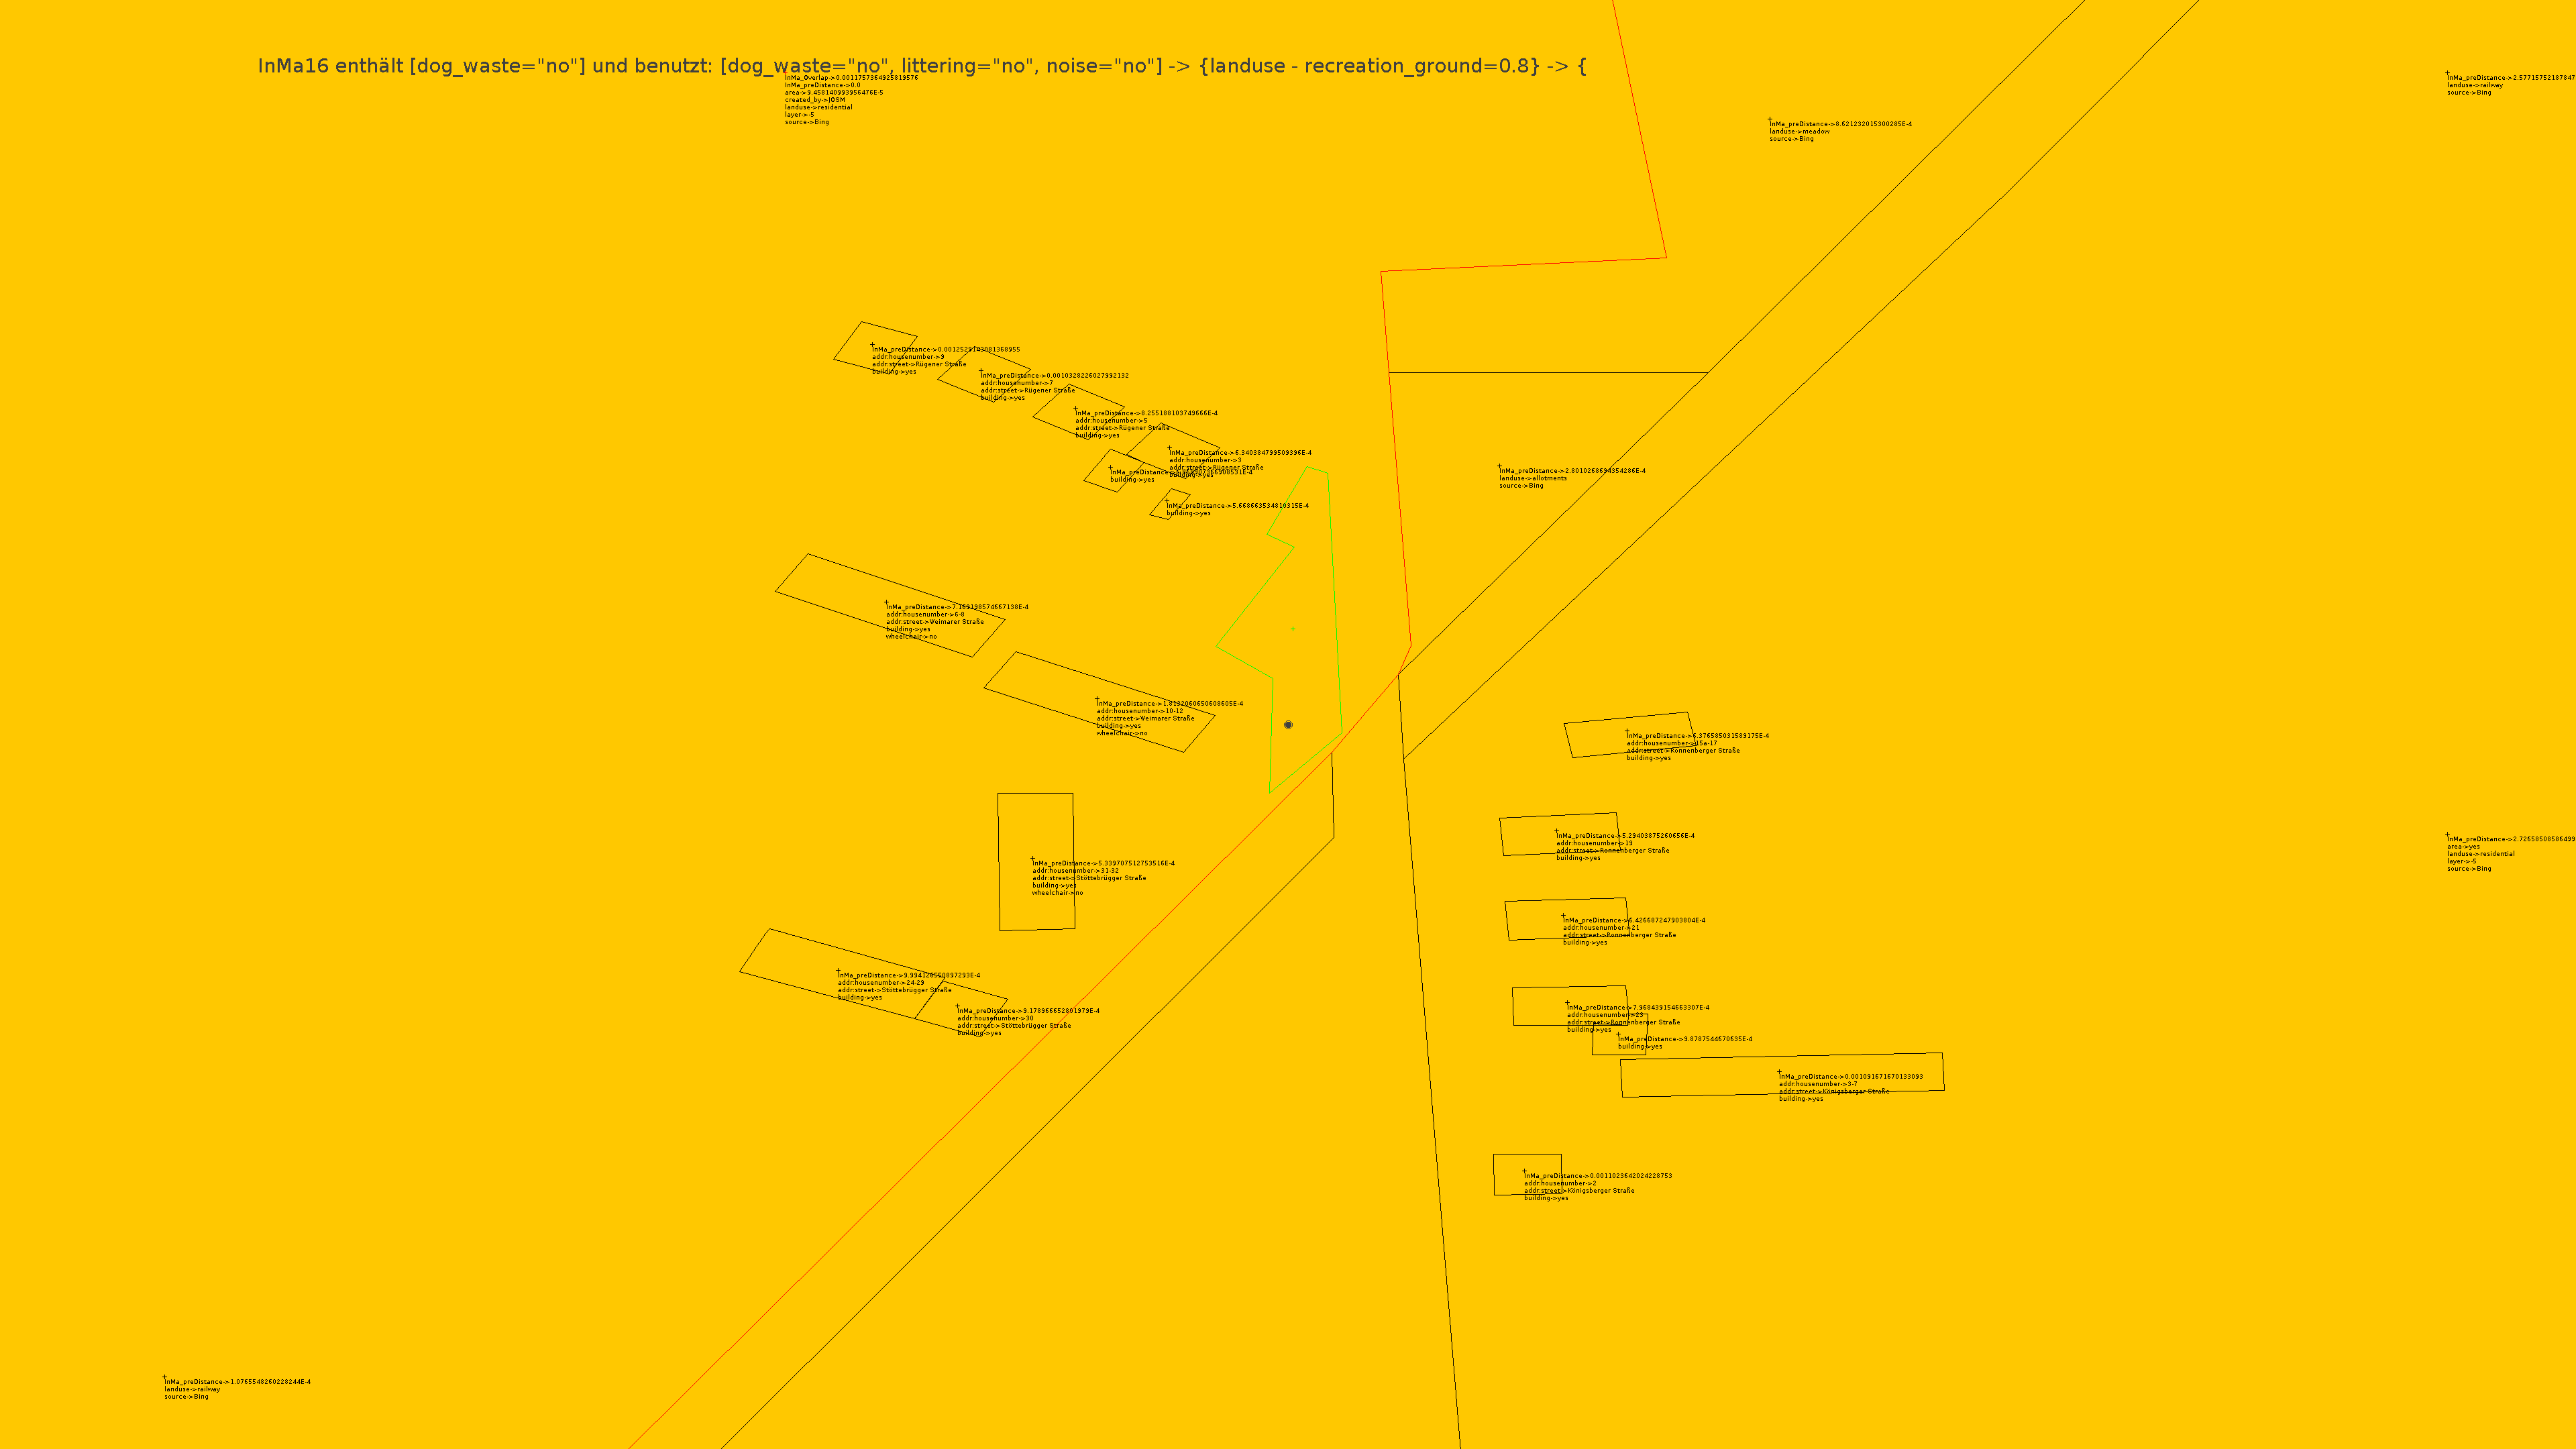
\includegraphics[width=\textwidth]{InMa16.png}
  \caption{Unvollständige Rules Einschränkungen.}
  \label{fig:MissingCircle}
\end{figure}
Das von uns bis jetzt definierte Regelwerk liefert nach einem ersten Durchlauf
zufriedenstellende Ergebnisse. Die Überlappungen sind meistens gegeben, jediglich
in 2 Fällen lag er komplett daneben. Dieses ist auf ein unvollständiges Regelwerk
aufgrund zu wenig Datansätzen zurück zu führen.

So gab es bis jetzt keine Definition für die Regel ''Zugang erst ab 21 Jahren''.
Dieses führte dazu, dass die Backup-Regel genommen wurde, das nächstebeste Polygon zu nehmen.
Da jedoch wie in \fref{fig:NoRule} zu sehen ist, das Bild vor dem gültigen Gebäude aufgenommen
wurde ist dem bisherigem Regelsatz nur noch die Regel:
\begin{lstlisting}[language=xml,frame=single]
<rule>
  <restriction>access:age="21+"</restriction>
  <OSMTag weight="0.8" >building</OSMTag>
</rule>
\end{lstlisting}

hinzuzufügen um auch diesen Datensatz vollständig zu bearbeiten.


Im zweiten Fall ist wie in \fref{fig:MissingCircle} zu sehen keine Representation
beabsichtigten Geltungsbereiches in OpenStreetMap vorhanden. Und auch wenn man davon
ausgehen kann, dass niemand gerne Hundkot vor der Nase hätte ist der beabsichtigte
Geltungsbereich für das Hinweisschild nur die Grünfläche, welche an den Parkplatz
und Strasse angrenzt.
Das Regelwerk ist also dahingehend zu ändern, dass folgende Regel hinzugefügt wird:
\begin{lstlisting}[language=xml,frame=single]
<rule>
  <restriction>dog_waste="no"</restriction>
  <OSMTag threshold="1e-8" radius="0.00023">landuse - residential</OSMTag>
</rule>
\end{lstlisting}
oder aber die bestehende Regel
\begin{lstlisting}[language=xml,frame=single]
<rule>
  <restriction>dog_waste="no"</restriction>
  <restriction>littering="no"</restriction>
  <restriction>noise="no"</restriction>
  <OSMTag weight="0.8" >landuse - recreation_ground</OSMTag>
</rule>
\end{lstlisting}
um den OSMTag erweitert wird.
Beides führt in diesem Fall zum gleichen Ergebnis.



\input{doc/doxyref}

% Index
\newpage
\phantomsection
\addcontentsline{toc}{chapter}{Index}
\printindex

\end{document}
